
\documentclass[natbib,doc,12pt,floatsintext]{apa6}
\usepackage{amsfonts, amsmath}
\usepackage{relsize}
\usepackage{epstopdf}
\usepackage{bm}
\usepackage{todonotes}
\usepackage{epigraph}
\usepackage{xcolor}
\usepackage{setspace}
\usepackage{graphicx}
\graphicspath{ {./images/} }
\definecolor{mypink}{RGB}{255, 230, 255}

%% begin custom commands
\newcommand{\J}[1]{\todo[inline, color=mypink ]{  #1 }}
\newcommand{\EJ}[1]{\todo[inline, color=green]{  #1 }}
%% end custom commands

\title{On the merits of specifying scientific questions}

\shorttitle{Jeffrey's Platitude}

\fourauthors{Julia M. Haaf}{Angelika M. Stefan}{Quentin Gronau}{Eric-Jan~Wagenmakers}
\fouraffiliations{University of Amsterdam}{University of Amsterdam}{University of Amsterdam}{University of Amsterdam}

\authornote{This research was supported by ... Correspondence should be sent to Julia M. Haaf, University of Amsterdam, Nieuwe Achtergracht 129 B, 1018 WT Amsterdam, The Netherlands. E-mail may be sent to j.m.haaf@uva.nl. \J{Add link to github/osf project?}}

\abstract{}

\keywords{Bayes factor, Bayesian model averaging}

\begin{document}

\onehalfspacing

\maketitle

\newpage

\section{Introduction}

\setlength{\epigraphwidth}{.8\textwidth} % set for individual epigraph
\epigraph{It is sometimes considered a paradox that the answer depends not only on the observations but on the question; it should be a platitude.}{Jeffreys, 1939, p.vi}

In many debates in psychological science we focus on the existence of psychological phenomena and size of the corresponding effects. This focus is reflected in the current debate around the reproducibility crisis. Many large-scale replication studies test whether an effect in the literature exists, and quantify this existence with evidence for a non-null alternative hypothesis \citep{OpenScienceCollaboration:2015, Ebersole:etal:2016}. This quantification is often done in the frequentist framework (i.e. $p<.05$), but Bayesian alternatives to quantify replication success have been proposed as well \citep{Verhagen:Wagenmakers:2014}.

This strong focus on the existence of an effect reflects the scientific question we most commonly address with statistical analysis: \textit{Is there an effect?} The is-there-an-effect question, however, is only one of many scientific questions we care about in psychological research. Psychological theories oftentimes provide additional ordinal constraint on data leading to the question of \textit{is there an effect in the pre-specified direction?} Furthermore, \cite{Haaf:etal:2019} argue that many psychological theories provide multiple ordinal constraints simultaneously. Such simultaneous constraints can lead to a range of scientific questions such as, "if X is constant across conditions, is Y larger in condition A than condition B?" 

With regards to the quote by \cite{Jeffreys:1939} above, the is-there-an-effect question, and the current focus on psychological phenomena translates to a focus on \textit{observations}. Here, we provide an exploration of the impact of scientific \textit{questions}. We present a taxonomy of the most common scientific questions in psychology, and show how different scientific questions can be translated into the comparison of statistical models. We then explore the effect of the choice of \textit{question} on the \textit{answer} of a scientific inquiry. This exploration illustrates that this effect of the \textit{question} on the \textit{answer} is not always intuitive. Researchers should choose both scientific question and translation to statistical models with utmost care.

\section{Taxonomy of Scientific Questions}

Many of the common scientific questions in psychology can be categorized as corresponding to one of two theoretical constraints. The first theoretical constraint is the equality constraint, and this theoretical consideration corresponds to the typical null hypothesis testing case. The second theoretical constraint is the ordinal constraint corresponding to one-sided tests. Figure~\ref{fig:questiontree} shows five scientific questions corresponding to these constraint that are used as most common examples throughout the paper. Note that some of these questions are generalizations and simplifications of one another, and there are many additional question formulations possible. Yet, they correspond to the most typical scientific questions psychologists try to answer.

\begin{figure}[h]
\caption{Connection between theoretical constraints, scientific questions, and instantiation of these questions as competing models.}
\centering
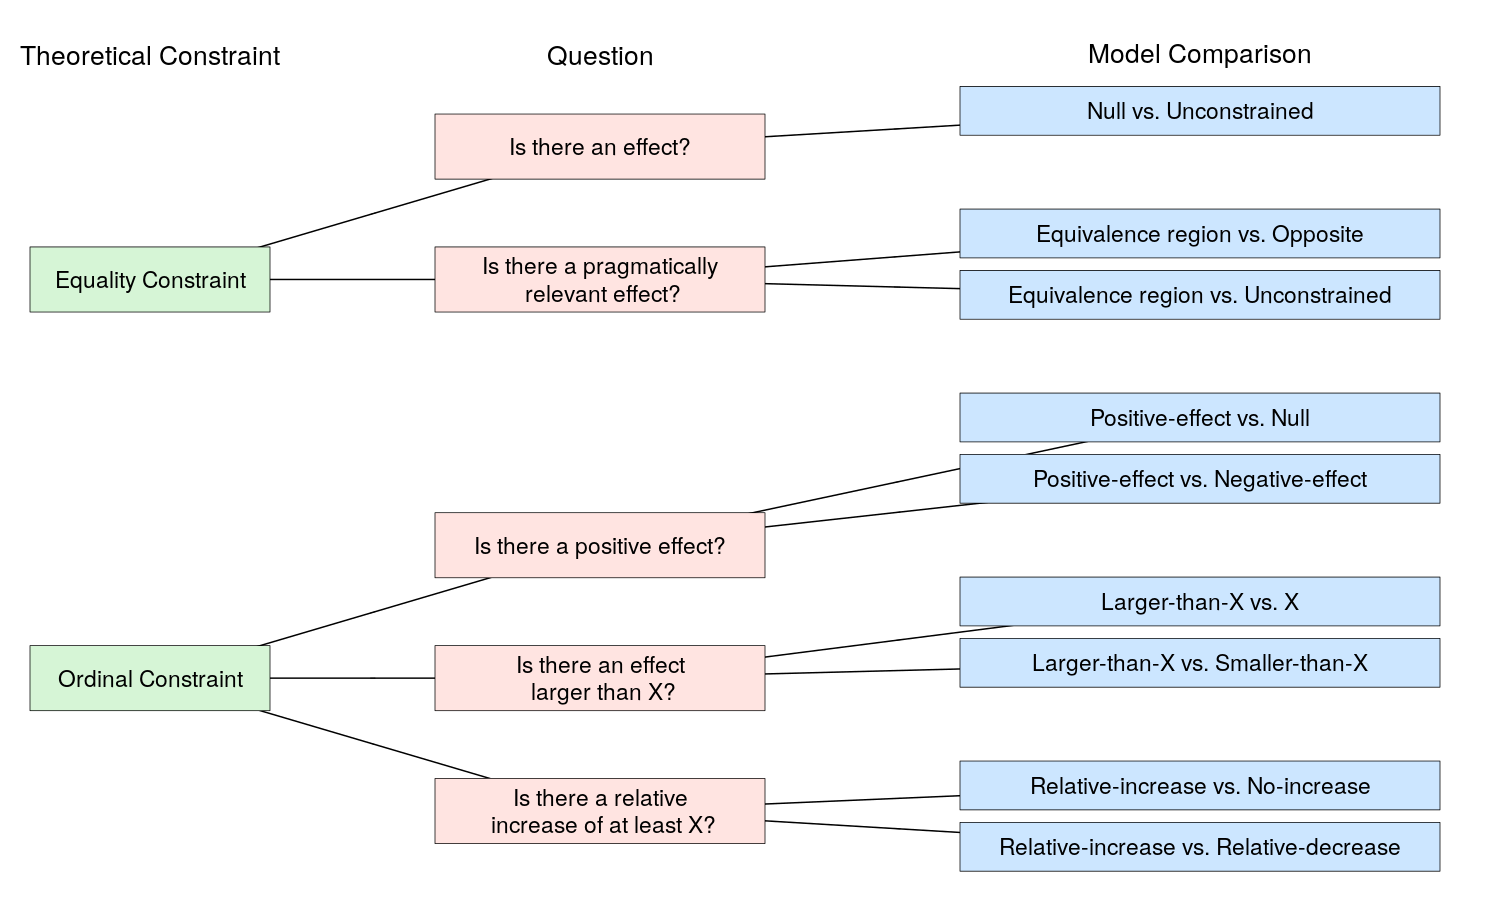
\includegraphics[width=1\textwidth]{questiontree.png}
\label{fig:questiontree}
\end{figure}

\subsection{Questions about Equality Constraints}

Scientific questions in this category are, for example, "is there an effect", or "is there an effect deemed meaningful". Here, we will briefly discuss the theoretical implications and utilization of these two exemplary questions.

The question whether there is an effect is probably the most common scientific question in the psychological literature. The question is a powerful question when the goal is to uncover invariance, or conversely, the violation of invariance. Especially the invariance (i.e. there is no effect) of a psychological phenomenon may have huge implications on psychological theory. Perhaps the main reason for the predominance of this question in the psychological literature is the current state of default statistical testing that mostly focusses on null hypothesis testing (CITE).

The question whether there is a meaningful effect is based on the assumption that no effect is ever truly zero \citep{Cohen:1994}. Therefore, asking whether there is an effect at all is not an interesting question to ask as the answer, yes, is already known \citep{Morey:Rouder:2011, Meehl:1978, Berger:Delampady:1987}. Instead, we may define a meaningful effect as an effect that is outside of pre-specified boundaries around zero \citep{Lakens:2017}. Which boundaries are specified depends on the field, the study design, and many other factors \citep{Lakens:etal:2018}. While the question whether there is a meaningful effect is not as popular, it recently gained traction with the implementation of easy-to-apply frequentist equivalence tests. 

In their core, the two questions have the same goal of uncovering invariances or their violation. A preference for one of these questions is typically based on convenience of analysis tools, the specific application, or the philosophical mindset. However, the questions, as discussed subsequently, may yield somewhat different scientific answers for the same setting. 

\subsection{Questions about Ordinal Constraints}

Scientific questions in this category are, for example, "is there an effect in the predicted direction", "is there an effect larger than x", where x is a set value, or "is the effect in one setting at least x times as large as in another setting", where, again, x is a set value. Here, we will briefly discuss the theoretical implications and utilization of these two exemplary questions.

Perhaps the most common ordinal constraint question is whether there is an effect in the predicted direction. This question corresponds, for example, to a predicted ordering of cell means for experimental conditions, or the direction of the relationship between two variables. Several authors have argued that questions about the direction of an effect more closely correspond to psychological theory than questions about the existence of an effect \citep{Gu:etal:2014, Haaf:etal:2019}.

A generalization of the question about the direction of an effect is whether the effect is larger than a set value. This question is suitable in domains where a specific value is important. In most of psychology, where conditions are contrasted or relationships between variables are assessed, the value of most importance is zero. Another often important value is chance performance, for example 50\% accuracy in a two-alternative-forced-choice paradigm. While we wanted to mention this generalization, we will use the special case of $x=0$ for illustration throughout the paper. Note that a comparable generalization can be made for the question whether there is an effect. Typically, we assume an effect means that the effect is not equal to zero. However, any other value could be specified. In the case of chance performance, we may define "no effect" as performance on chance level. 

Another ordinal constraint of interest may be... \J{Quentin, Angelika, we talked about this question: Is the effect in condition A at least X times as large as in condition B? Can anybody come up with an example where this may be useful?}

\subsection{Combinations}

Any of these questions can be investigated in combination, and any specific scientific question can have any number of these components. 

\section{Translating Scientific Questions into Model Comparison}

\subsection{Visualizing predictions from statistical models}

\begin{itemize}
    \item Priors as predictive device
\end{itemize}

\section{Applications}

A combination of 2 applications would be useful to illustrate how results change depending on the question. The first application is for the contrast between two conditions in an experiment (t-test). We can explore the effect of sample size on the different Bayes factors. The second application is one where the number of constraints increases with sample size (such as "does everyone", or multinomial test). What is the effect of question then?

\J{Unlike Bayesian prior settings that get washed out by lots and lots of data, the effect of the question is at least constant. This effect may sometimes even increase with N? If so, when would it increase? Would be nice to show that.}

\subsection{Is there a priming effect?}

Possible Questions:

\begin{itemize}
    \item \textit{Is there an effect?} Null vs. unconstrained alternative
    \item \textit{Is there an effect such that people are faster if prime valence and target valence match?} Null vs. one-sided alternative (vs. other-sided or unconstrained alternative)
    \item \textit{Is the effect non-equivalent to zero?} Equivalence region vs. alternative (either constrained or unconstrained)
\end{itemize}

\subsection{Is the priming effect stable across participants?}

\section{Considerations of sample size and study planning}

\section{Discussion}

\begin{itemize}
    \item What types of questions can I ask?
    \item How many models should be compared?
    \item How can we interpret the comparison?
\end{itemize}

\clearpage
\bibliography{lab}

\end{document}
